\documentclass[12pt]{article}

\usepackage{hyperref}
\usepackage{tikz}
\usepackage{pgfplots}

\title{Security Analysis of Telegram \\
    \large 6.857 Final Project}
\author{Hayk Saribekyan (hayks@mit.edu) \\
        Akaki Margvelashvili (margvela@mit.edu)}
\date{\today}

\begin{document}
    \maketitle
    
    \begin{abstract}
        Telegram is an instant text messaging platform, with a secure messaging protocol called MTProto. The company was founded in 2013 and has more than 100 million active users. Telegram was created to allow users to have surveillance-proof communication. It claims to have the best security and privacy guarantees in the market. In this report we overview Telegram, discuss its protocol and compare it to similar products. We also exploit a leak on user availability and use it to predict when users are talking to each other.
    \end{abstract}
    
    \section{Introduction}
    
    % talk about messaging, telegram and other similar products
    In the past decade, as more and more people got access to the internet, instant messaging services have thrived. As of May 2017, two of the top five most downloaded applications on Android market are messaging services \cite{androidrank}.
    In recent years the users of communication tools, including messaging services, have become more conscious about the privacy and security concerts. To suit the users' needs better, many platforms started offering end-to-end encryption \cite{facebook-secret,whatsapp-secret}. WhatsApp\footnote{Which, by the way, is down at the time of writing :) }, for example, introduced end-to-end encryption three years ago and as of now it is enabled for all its communications. It has the largest user base that has end-to-end encryption enabled for everyone. Despite this, WhatsApp TODO had issues with authentication.
    
    Among many messaging services is Telegram, which has been founded in 2013. Despite being a newcomer to the field, it has more than 100 million monthly users, especially in Eastern Europe. Telegram claims to have the best security and privacy guarantees among similar products, but relies on the users to trust it by the virtue of its history and talent. For our project, we would like to perform a security analysis of Telegram \cite{telegram}, as it has come under heavy fire from many professional cryptographers due to its unorthodox decisions in development.
    
    In this section, we will discuss Telegram's history and user interface. Section \ref{sec:policy} describes Telegram's security policy; Section \ref{sec:mtproto} describes their own secure messaging protocol; Section \ref{sec:issues} contains previously known issues with Telegram; Sections \ref{sec:availability} and \ref{sec:results} discuss a privacy vulnerability that Telegram exposes. In Section \ref{sec:conclusion} we reflect on Telegram and draw conclusions.
    
    \subsection{History and Background}
    % Telegram's popularity wouldn't be as it is if not its history, so we need to talk about it

    Telegram's history is unique among tech stratups and we believe that it gained much attention, trust and user base thanks to that. So it is worth to mention the history as a background.
    
    Telegram was founded in 2013 by brothers Nikolai and Pavel Durov, who was also the founders of a popular Russian social network VK. After pressure from the Russian government to hand over backdoors Durov left the company and claimed that VK is under control of the political party in power \cite{durov-fired}. He then left Russia and founded Telegram, aiming to provide surveillance-proof messaging to non-tech-savvy users.
    
    Thanks to Pavel Durov's popularity in Russia, Telegram quickly gained ground among Russian-speaking community. Moreover, Telegram arguably provides one of the best user experiences compared to similar products thanks to its speed and functionality.

    Telegram's messaging protocol is developed by Pavel's brother Nikolai, who is a mathematician, but is not known as a security expert.
    
    Telegram is unique among tech startups in that its solve funding source is the founder Pavel Durov. It does not use adds anywhere on its platform and the clients are not only free, but also open-source.
    
    \subsection{Telegram Functionality}
    Telegram allows users to send instant messages, voice messages and communicate in groups. It also has 'channels', to which users can subscribe and receive broadcast messages by the creator of the channel (usually a news website or a celebrity).
    
    Telegram has a 'secret chat' feature, which is not enabled by default. The secret chats are Telegram's version of end-to-end encryption. The messages are destroyed after a time limit set by the user and should not recoverable. Telegram has chosen to not make messages end-to-end encrypted by default to enhance user experience: secret chats are bound to specific devices and it is impossible to continue a conversation on a device it was not started on.
    
    Users in Telegram have to create and authenticate their accounts using an authentication code received by text messages. After the initial authentication, the users can set handles and find each other using those. Telegram also has a two-step verification mechanism for which the user has to enter a password every time s/he authenticates.
    
    \subsection{Telegram Clients}
    % add a screenshot from desktop and mobile apps
    Telegram has clients for all popular platforms including web applications. Figure \ref{fig:ui-clients} shows Telegram's clients for Android and Desktop. The official clients are open-source though they have binary blobs i.e. executable binaries without publicly available codes.
    
    \begin{figure}
        \centering
        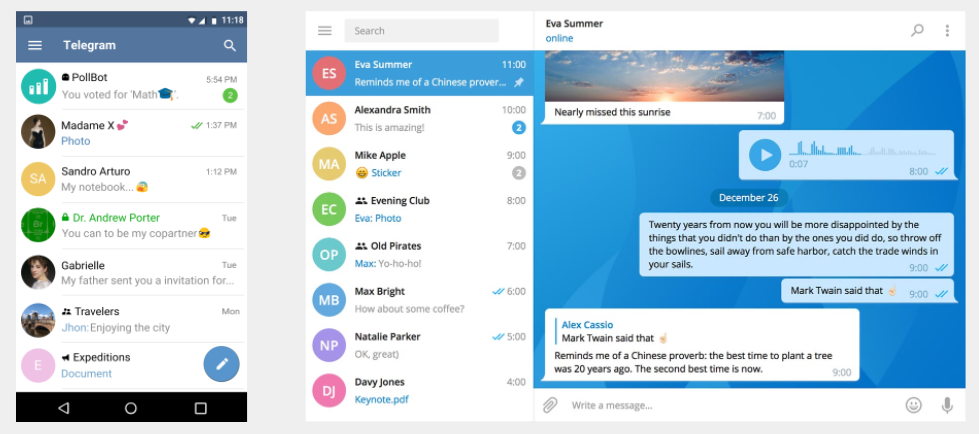
\includegraphics[width=\textwidth]{clients.png}
        \caption{Official Telegram clients. Left: mobile client, right: desktop client. All official Telegram clients are open-source. Telegram provides noticeable faster and smoother user experience.}
        \label{fig:ui-clients}
    \end{figure}
    % mention the command line client and write about it
    
    Telegram even has a command line interface \cite{telegram-cmd}, which provides almost full functionality of the messaging platform albeit it is not as user-friendly. For example, to add a contact one has to write in the interface \\
    \texttt{tg> add\_contact <phone\_number> <name> <lastname>}\\
    We have extensively used the command line interface during this project.
    
    \section{Telegram Security Policy}
    \label{sec:policy}
    
    % actors, server, etc (see lecture, and other projects)
    This section briefly describes the security policies of Telegram messenger.

    % say that some of the stuff it exposes but it should not    
    \section{MTProto}
    \label{sec:mtproto}
    
    % bring in the picture of MTProto, paraphrase from their webiste
    
    
    \section{Known and Fixed Security Issues}
    \label{sec:issues}
    
    \section{Availability Exploit}
    \label{sec:availability}
    
    % describe on high level
    
    \subsection{Experiment Setup}
    % used the command line client
    % had N users
    % were listening all day long for a week
    
    % screenshot from the command line interface.
    
    \subsection{Correlation Algorithm}
    
    % need to find a paper that maybe does something like this, and use it. Citations are good
    
    \section{Results from Availability Exploit} % maybe a subsection, then just "Results"
    \label{sec:results}
    
    % pretty graphs 
    
    \section{Conclusion}
    \label{sec:conclusion}
    
    \bibliographystyle{unsrt}
    \bibliography{references}

\end{document}
